%% This is an example first chapter.  You should put chapter/appendix that you
%% write into a separate file, and add a line \include{yourfilename} to
%% main.tex, where `yourfilename.tex' is the name of the chapter/appendix file.
%% You can process specific files by typing their names in at the 
%% \files=
%% prompt when you run the file main.tex through LaTeX.

\singlespacing{

\chapter{Future Work}\label{chap:futureWork}

Future work revolves around extensions of the current simulation model, 
setting up for experiments in computational design optimization.

\section{Hierarchical Simulation}

\begin{figure}
  \includegraphics[width=\textwidth]{FunctionsParts.png}
  \caption{}
  \label{fig:FunctionsParts}
\end{figure}

\begin{figure}
  \includegraphics[width=\textwidth]{HierarchicalSim.png}
  \caption{}
  \label{fig:HierarchicalSim}
\end{figure}

Increasing levels of hierarchy correspond to increased simulation abstraction
Higher levels of hierarchy exhibit high-level behaviors which are abstracted from the low level physics of the system.

\section{"Fab the Game"}

An offshoot of the work described in this thesis is a collaboration with \href{http://elinemedia.com/}{E-Line Media} on a game that explores an aspirational future where digital materials are used to construct nearly everything.  Tentatively called "Fab the Game", 

Players construct assemblies from functional primitives in an open-ended sandbox environment and in more directed challenges.  We envision a large component of gameplay revolves around constructing robots and using them to interact with and shape the surrounding environment.


Robots which are controlled in real time by players to compete in arena challenges, drawing inspiration from the competitions of \href{http://www.firstinspires.org/robotics/frc}{First Robotics}.


Players can dive into functional primitive definitions and alter the elemental composition to alter its function-level behavior.  Advanced gameplay involves designing new functional primitives from elemental part types to achieve behaviors beyond those provided by default.  We hope to encourage gameplay similar to what I've described exists around the Game of Life in Chapter \ref{chapter:HierarchicalDesign} and allow greater interaction with research at CBA.

Concept art by Eli Gershenfeld explores the look and feel of the game as well as potential gameplay scenarios (Figures \ref{fig:elibendy} through \ref{fig:elibridgefull}).

\begin{figure}
  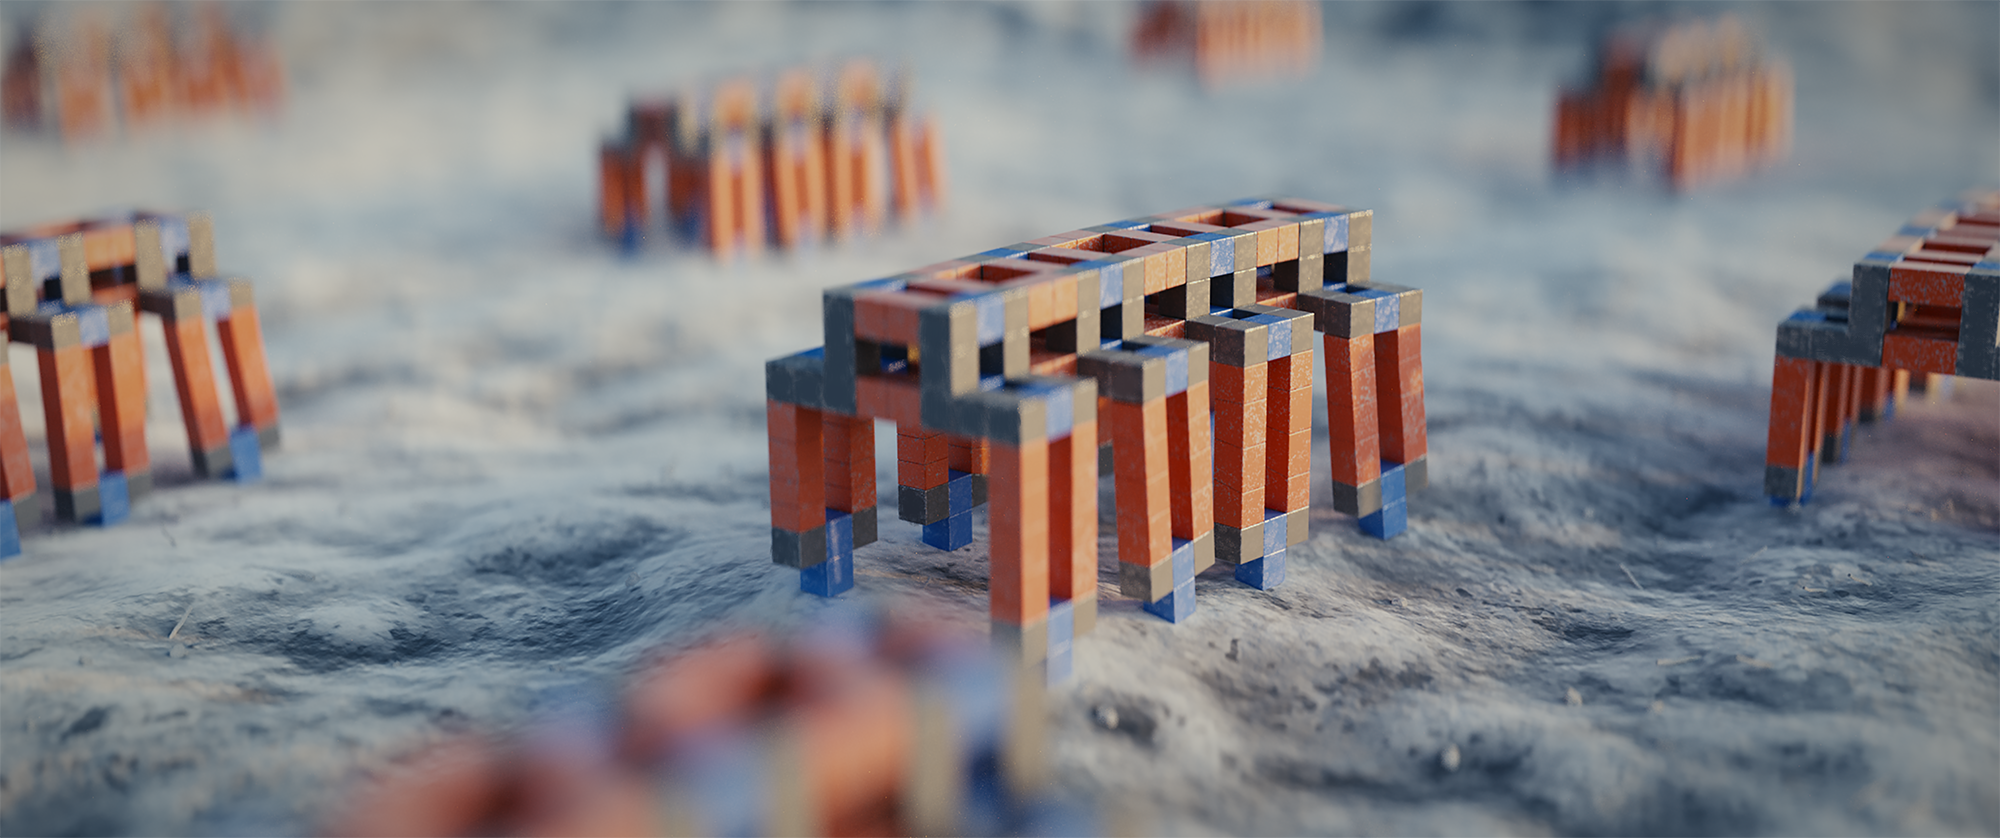
\includegraphics[width=\textwidth]{elibendy.png}
  \caption{A swarm of locomoting robots.  \textit{Image Credit: Eli Gershenfeld 2016}}
  \label{fig:elibendy}
\end{figure}

\begin{figure}
  \includegraphics[width=\textwidth]{eliassemblers.png}
  \caption{Assembler assembling an assembler.  \textit{Image Credit: Eli Gershenfeld 2016}}
  \label{fig:eliassemblers}
\end{figure}

\begin{figure}
  \includegraphics[width=\textwidth]{eliassembclose.png}
  \caption{Assembler "factory" feedstock.  \textit{Image Credit: Eli Gershenfeld 2016}}
  \label{fig:eliassembclose}
\end{figure}

\begin{figure}
  \includegraphics[width=\textwidth]{eliassembwide.png}
  \caption{Distributed "factory" automation. \textit{Image Credit: Eli Gershenfeld 2016}}
  \label{fig:eliassembwide}
\end{figure}

\begin{figure}
  \includegraphics[width=\textwidth]{elibridgeclose.png}
  \caption{"Living" macro-scale structure.  \textit{Image Credit: Eli Gershenfeld 2016}}
  \label{fig:elibridgeclose}
\end{figure}

\begin{figure}
  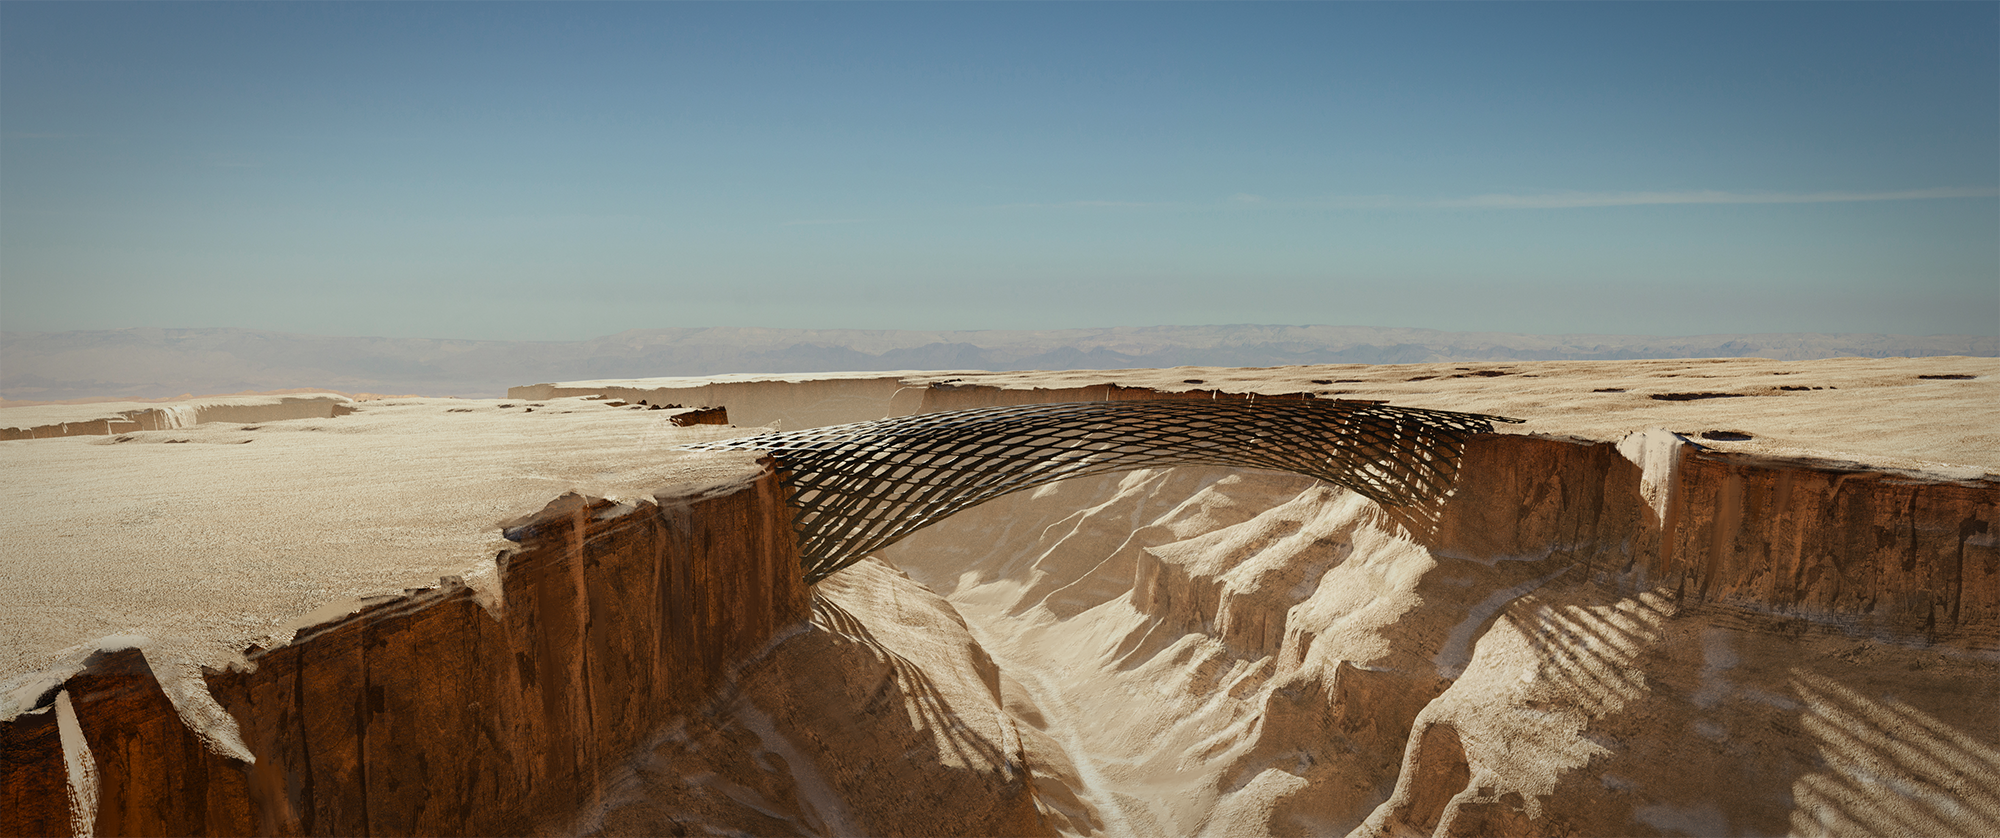
\includegraphics[width=\textwidth]{elibridgefull.png}
  \caption{Self-assembling bridge. \textit{Image Credit: Eli Gershenfeld 2016}}
  \label{fig:elibridgefull}
\end{figure}

\section{Computational Design Optimization}

Sets up nicely for computational design optimization

Contrained design space, due to the discretization of space and a limited set of potential parts types.

Low hanging fruit involves implementation of the element $\rightarrow$ functional primitive simulation and topological optimization of the patterning of elemental parts.
